\section{Prepogibanje stožnic}
\label{pogl:stoznice}

% kako konstruiramo tangente na stožnice in zakaj konstrukcije tako delujejo
% parabola, elipsa, hiperbola
% povezava z O6
% pa omeni tudi O7, kjer je skupna tangenta na dve paraboli
% a za krožnico se tudi da?

Iz didaktičnega vidika zelo zanimivo poglavje nam predstavlja konstrukcije tangent na stožnice s prepogibanjem papirja. Vsebina je tu predstavljena tako, da je bralec najprej povabljen, da vzame list papirja in ga prepogiba po navedenih korakih. Po opažanju, kaj se na papirju po tem prikaže, preidemo na matematični del, kjer dokažemo, da so prepogibi res tangente na določeno stožnico.

% Za vsako stožnico:
% 1. konstrukcija (navodila za prepogibanje)
% 2. matematični dokaz, zakaj so to ravno tangente
% kdo je izumil ta navodila in kdaj?
% je še kakšna druga metoda?

% na koncu še O7 -- konstrukcija skupne parabole na dve stožnice -- a se da iz tega še kaj pametnega izcimit?

\subsection{Parabola}

% Hull je našel Row-a (prvič izdana 1893) kot najstarejši zapis te konstrukcije
\textit{\textbf{Naloga:} Vzemi pravokoten list papirja in svinčnik ter opravi naslednje korake (gl. tudi sliko~\ref{fig:koraki_parabola}):
\begin{enumerate}
    \item \label{korak1} Nekje sredi spodnje polovice lista s pisalom označi točko.
    \item \label{korak2} Na spodnji stranici lista si izberi točko in list prepogni tako, da se obe izbrani točki prekrijeta.
    \item \label{korak3} Ponovi korak~\ref{korak2} za drugo točko na spodnji stranici.
\end{enumerate}
Kaj opaziš po večkratni ponovitvi koraka~\ref{korak2}?}

\begin{figure}[h]
    \centering
    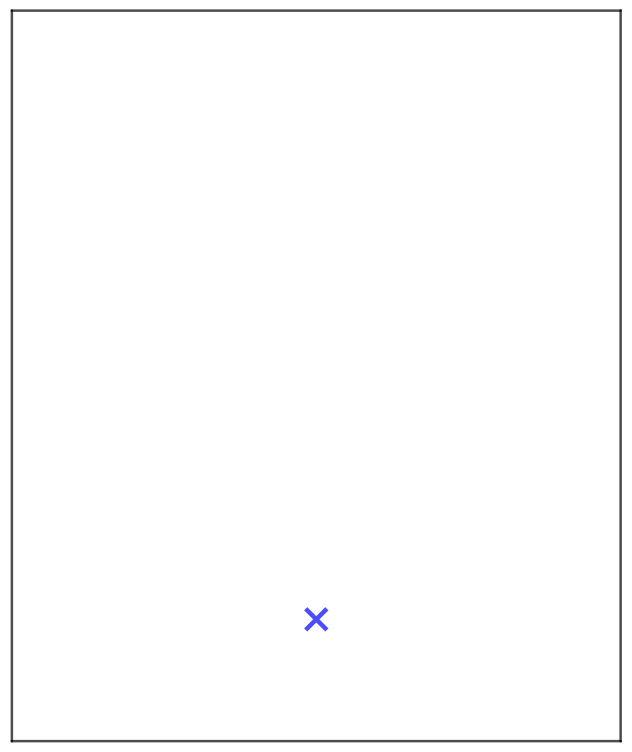
\includegraphics[width=0.3\textwidth]{images/stožnice/folding_parabola_1.png}
    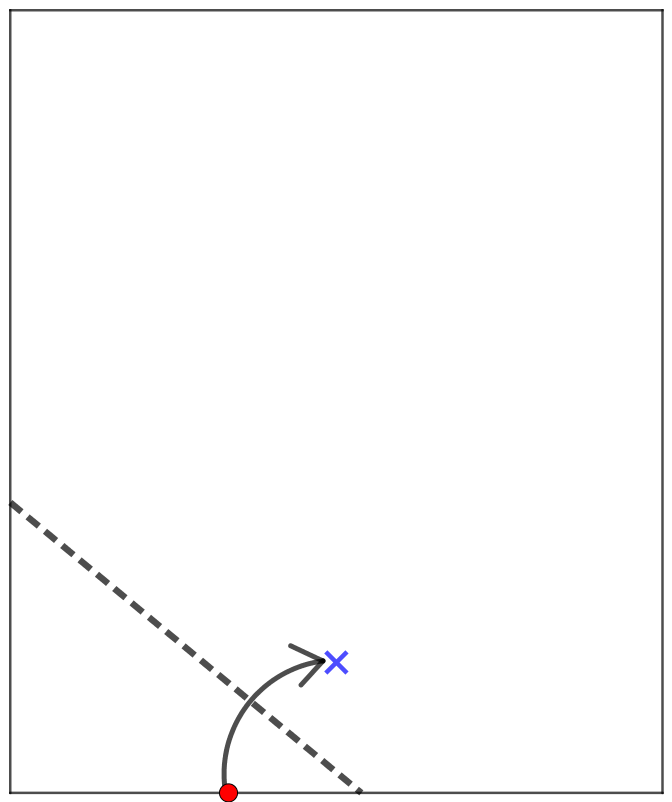
\includegraphics[width=0.3\textwidth]{images/stožnice/folding_parabola_2.png}
    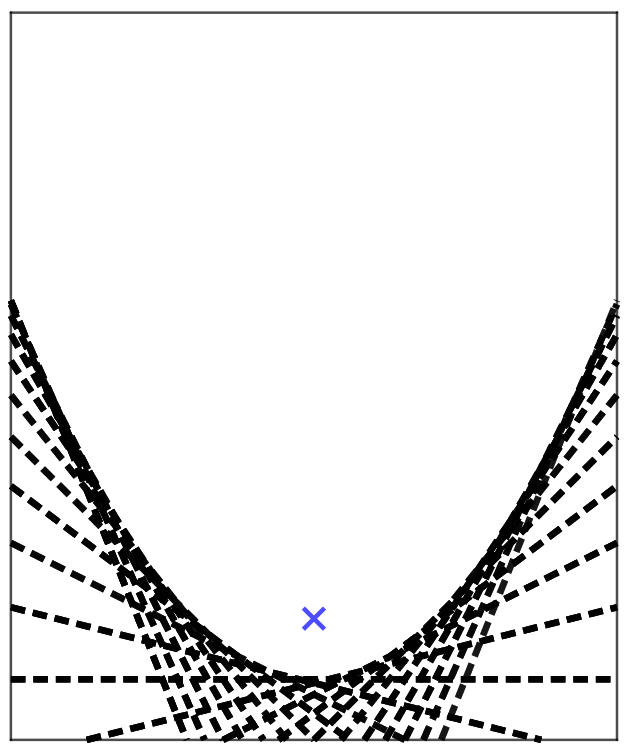
\includegraphics[width=0.3\textwidth]{images/stožnice/folding_parabola_3.png}
    \caption[Prepogibanje parabole]{Prepogibanje parabole po korakih (iz leve proti desni)~\ref{korak1},~\ref{korak2} in~\ref{korak3}.}
    \label{fig:koraki_parabola}
\end{figure}

Korak~\ref{korak2} je deloma operacija~\ref{op:O6}, ki smo jo spoznali v poglavju~\ref{pogl:aksiomi}. Tam smo že premislili, da nam pregib premice $a$ na točko $A$, ki poteka skozi dano točko $B$, poda tangento na parabolo z goriščem $A$ in premico vodnico $a$ (gl.\ sliko~\ref{fig:O6_parabola} in premislek nad njo). Tukaj pa v koraku~\ref{korak2} točke $B$ ne vključimo, saj je katerikoli pregib, ki premico $a$ položi na točko $A$, neka tangenta na taisto parabolo -- pregib je namreč simetrala daljice, ki ima za krajišči obe točki iz korakov~\ref{korak1} in~\ref{korak2}, torej obstaja točka, ki je enako oddaljena od spodnje stranice papirja in na koraku~\ref{korak1} izbrane točke (točka $P$ na sliki~\ref{fig:O6_parabola}). Nadaljni premislek, da je to edino presečišče pregiba in parabole, pa je enak kot prej.

Po večkrat izvedenih pregibih spodnje stranice lista na začetno izbrano točko dobimo na papirju obris parabole.